% Graphics for slide 23, in the order the PDF draws them.
\begin{tikzpicture}[remember picture, overlay, x=1bp, y=-1bp,
  shift={(current page.north west)}]
\path[fill=cFFFFFF] (0,0) rectangle (960,540);
\node[anchor=north west, inner sep=0pt] at (420.06,234.96) {
\includegraphics[width=117.94bp, height=117.94bp]{figures/fundamentals-of-hpc/p23-1.png}};
\path[draw=cFFFFFF,line width=1.25bp,line join=round] (365.8,228.36) --(592.34,228.36) --(594.98,228.54) --(597.47,229.06) --(599.73,229.89) --(601.71,231) --(603.37,232.35) --(604.64,233.93) --(605.45,235.71) --(605.73,237.59) --(605.73,359.36) --(352.41,359.36) --(352.41,237.59) --(352.69,235.71) --(353.5,233.93) --(354.77,232.35) --(356.43,231) --(358.41,229.89) --(360.67,229.06) --(363.16,228.54) --(365.8,228.36);
\node[anchor=north west, inner sep=0pt] at (118.45,232.94) {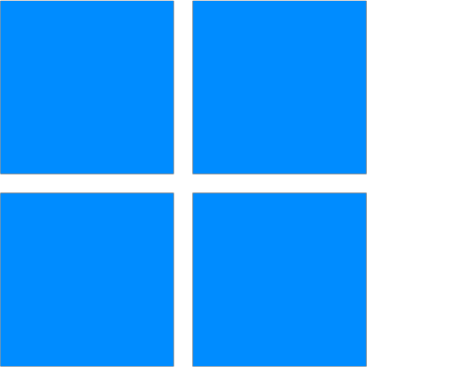
\includegraphics[width=154.98bp, height=121.94bp]{figures/fundamentals-of-hpc/p23-2.png}};
\node[anchor=north west, inner sep=0pt] at (56.69,477.21) {
\includegraphics[width=73.42bp, height=37.42bp]{figures/fundamentals-of-hpc/p03-1.png}};
\path[fill=cEE7628,even odd rule] (57.18,55.73) ..controls(57.96,55.73)and(58.6,56.37)..(58.6,57.15) --(58.6,85.5) ..controls(58.6,86.28)and(57.96,86.91)..(57.18,86.91) ..controls(56.4,86.91)and(55.76,86.28)..(55.76,85.5) --(55.76,57.15) ..controls(55.76,56.37)and(56.4,55.73)..(57.18,55.73);
\node[anchor=north west, inner sep=0pt] at (724.73,234.36) {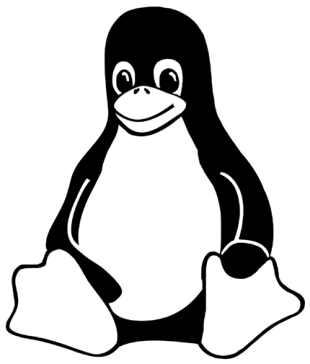
\includegraphics[width=103.14bp, height=121.02bp]{figures/fundamentals-of-hpc/p23-4.png}};
\path[fill=cF6DA44,even odd rule] (66.05,456.18) --(297.48,456.18) ..controls(303.16,456.18)and(307.76,451.57)..(307.76,445.89) --(307.76,358.74) --(55.76,358.74) --(55.76,445.89) ..controls(55.76,451.57)and(60.37,456.18)..(66.05,456.18);
\path[fill=cF6DA44,even odd rule] (363.32,456.18) --(594.75,456.18) ..controls(600.43,456.18)and(605.03,451.57)..(605.03,445.89) --(605.03,358.74) --(353.03,358.74) --(353.03,445.89) ..controls(353.03,451.57)and(357.64,456.18)..(363.32,456.18);
\path[fill=cF6DA44,even odd rule] (660.59,456.18) --(892.02,456.18) ..controls(897.7,456.18)and(902.3,451.57)..(902.3,445.89) --(902.3,358.74) --(650.3,358.74) --(650.3,445.89) ..controls(650.3,451.57)and(654.91,456.18)..(660.59,456.18);
\path[fill=c2CA055,even odd rule] (56.69,170.25) ..controls(56.69,167.62)and(58.82,165.49)..(61.45,165.49) --(897.54,165.49) ..controls(900.17,165.49)and(902.3,167.62)..(902.3,170.25) --(902.3,189.29) ..controls(902.3,191.92)and(900.17,194.05)..(897.54,194.05) --(61.45,194.05) ..controls(58.82,194.05)and(56.69,191.92)..(56.69,189.29) --(56.69,170.25);
\end{tikzpicture}
